\documentclass[9pt]{article}
\usepackage[utf8]{inputenc}
\usepackage{geometry}
\geometry{letterpaper, margin=0.25in}
\usepackage{graphicx} 
\usepackage{multicol}
\usepackage{parskip}
\usepackage{booktabs}
\usepackage{array} 
\usepackage{paralist} 
\usepackage{verbatim}
\usepackage{sectsty}
\usepackage[shortlabels]{enumitem}

\usepackage{amsmath}
\usepackage{amssymb}
\usepackage{mathtools}
\usepackage{empheq}
\usepackage{xcolor}
\usepackage{bbm}
\usepackage{tikz}
\usepackage{pgfplots}
\usepackage{tikz-cd}
\usepackage{circuitikz}
\usepackage{multirow}
\pgfplotsset{compat=1.18}
\usetikzlibrary{intersections, decorations.markings}
\tikzset{
    marking along/.style n args={2}{
        decoration={
                markings, 
                mark=at position #1 with {\arrow{#2}}
        },
        postaction={decorate}
        },
    marking along/.default={0.5}{>}
    wavy/.style={
        decorate,decoration={coil,aspect=0}
     },
    two marks/.style n args={1}{
        decoration={
            markings,
            mark=at position 0.25 with {\arrow{#1}},
            mark=at position 0.75 with {\arrow{#1}}
         },
         postaction={decorate}
    }
    two marks/.default={>}
}

\colorlet{mygreen}{green!50!teal}
\colorlet{darkblue}{blue!60!black}

\newcommand{\ans}[1]{\boxed{\text{#1}}}
\newcommand{\vecs}[1]{\langle #1\rangle}
\renewcommand{\hat}[1]{\widehat{#1}}

\renewcommand{\P}{\mathbb{P}}
\newcommand{\R}{\mathbb{R}}
\newcommand{\E}{\mathbb{E}}
\newcommand{\Z}{\mathbb{Z}}
\newcommand{\N}{\mathbb{N}}
\newcommand{\Q}{\mathbb{Q}}
\newcommand{\C}{\mathbb{C}}

\newcommand{\ind}{\mathbbm{1}}
\newcommand{\qed}{\quad \blacksquare}

\newcommand{\brak}[1]{\left\langle #1 \right\rangle}
\newcommand{\bra}[1]{\left\langle #1 \right\vert}
\newcommand{\ket}[1]{\left\vert #1 \right\rangle}

\newcommand{\abs}[1]{\left\vert #1 \right\vert}
\newcommand{\mfX}{\mathfrak{X}}
\newcommand{\ep}{\varepsilon}

\newcommand{\Ec}{\mathcal{E}}
\newcommand{\Nc}{\mathcal{N}}
\newcommand{\A}{\mathcal{A}}
\newcommand{\F}{\mathcal{F}}
\newcommand{\Cc}{\mathcal{C}}
\newcommand{\B}{\mathcal{B}}
\newcommand{\M}{\mathcal{M}}
\newcommand{\X}{\chi}
\renewcommand{\L}{\mathcal{L}}

\newcommand{\sub}{\subseteq}
\newcommand{\st}{\text{ s.t. }}
\newcommand{\card}{\text{card }}
\renewcommand{\div}{\vspace*{10pt}\hrule\vspace*{10pt}}
\newcommand{\surj}{\twoheadrightarrow}
\newcommand{\inj}{\hookrightarrow}
\newcommand{\biject}{\hookrightarrow \hspace{-8pt} \rightarrow}
\renewcommand{\bar}[1]{\overline{#1}}
\newcommand{\overcirc}[1]{\overset{\circ}{#1}}
\newcommand{\diam}{\text{diam }}
\newcommand{\iid}{\overset{	ext{iid}}{\sim}}

\renewcommand{\Re}{\text{Re}\,}
\renewcommand{\Im}{\text{Im}\,}
\newcommand{\Var}{\text{Var}\,}
\newcommand{\Cov}{\text{Cov}\,}

\DeclareMathOperator*{\argmax}{\arg\max}
\DeclareMathOperator*{\argmin}{\arg\min}

\newcommand{\sign}{\text{sign}\,}

\newcommand*{\tbf}[1]{\ifmmode\mathbf{#1}\else\textbf{#1}\fi}

\usepackage{tcolorbox}
\tcbuselibrary{breakable, skins}
\tcbset{enhanced}
\newenvironment*{tbox}[2][gray]{
    \begin{tcolorbox}[
        parbox=false,
        colback=#1!5!white,
        colframe=#1!75!black,
        breakable,
        title={#2}
    ]}
    {\end{tcolorbox}}

\newenvironment*{exercise}[1][red]{
    \begin{tcolorbox}[
        parbox=false,
        colback=#1!5!white,
        colframe=#1!75!black,
        breakable
    ]}
    {\end{tcolorbox}}

\newenvironment*{proof}[1][blue]{
\begin{tcolorbox}[
    parbox=false,
    colback=#1!5!white,
    colframe=#1!75!black,
    breakable
]}
{\end{tcolorbox}}
\newenvironment*{proposition}[1][gray]{
    \begin{tcolorbox}[
        parbox=false,
        colback=#1!5!white,
        colframe=#1!75!black,
        breakable
    ]}
    {\end{tcolorbox}}


\begin{document}
\begin{multicols}{2}

\tbf{Linear system:} $L[au + bv] = aL[u] + bL[v], \quad a, b \in \R$

\tbf{LTI:} $y(t) = L[x(t)] \implies y(t - t_0) = L{x(t - t_0)}$

\tbf{Delta function:}
\begin{enumerate}
    \item $\int \delta(t)\; dt = 1$
    \item $\delta(t) = 0$ for $t \neq 0$
    \item $\int f(t) \delta(t - t_0)\; dt = f(t_0)$ (sifting)
\end{enumerate}

\tbf{Impulse response:} the output of an LTI system when the input is $\delta(t)$

\tbf{Transfer function:} $H(f) = \F(h(t))$ where $h(t)$ is the impulse response of the system.

\begin{center}
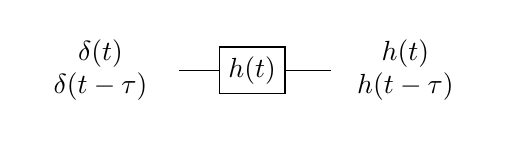
\begin{tikzpicture}
    \node at (0, 0) {\begin{tabular}{c}
        $\delta(t)$\\ 
        $\delta(t - \tau)$ 
    \end{tabular}};
    \draw (1, 0) -- ++(0.5, 0) node[right, draw, rectangle] (A) {$h(t)$};
    \draw (A) -- ++(1, 0) node[right] {\begin{tabular}{c}
        $h(t)$\\ 
        $h(t - \tau)$
    \end{tabular}};
\end{tikzpicture}
\end{center}
where the box represents a \tbf{convolution}:
\[y(t) = (x * h)(t) = \int_{-\infty}^\infty x(\tau) h(t - \tau) \; d\tau
\]
(in fact, in the frequency domain, this operation is defined by $Y(f) = X(f) H(f)$)

\tbf{Fourier Transform:} $\F[x(t)] = \int x(t)e^{-j\; 2\pi ft} \; dt = X(f)$

\tbf{Inverse Fourier:} $\F^{-1}[X(f)] = \int X(f) e^{j \; 2\pi ft} \; df = x(t)$

\emph{Standard Fourier pairs:}
\begin{enumerate}
    \item $\F[\delta(t)] = 1$
    \item $\F[e^{-j\; 2\pi f_0 t}] = \delta(f + f_0)$
    \item $\F[\delta(t- t_0)] = e^{-j\; 2\pi f t_0}$
    \item $X(f - f_0) = x(t) e^{j\; 2\pi f_0 t}$
    \item $\F[\cos 2\pi f_0 t] = \frac{1}{2}[\delta(f + f_0) + \delta(f - f_0)]$
    \item $\F[\sin 2\pi f_0 t] = \frac{1}{2j}[\delta(f + f_0) - \delta(f - f_0)]$
    \item $\F[\ind_{x\in [-T/2, T/2]}] = \text{sinc}(2\pi Tf)$
\end{enumerate}

\emph{Fourier Properties:}
\begin{enumerate}
    \item $\F[x(t - t_0)] = e^{-j\; 2\pi f t_0} X(f)$
    \item $\F[x(at)] = \frac{1}{\abs a}X(f/a)$
    \item $\F[x'(t)] = X(f) \cdot j\; 2\pi f$
    \item $\F[\int_{-\infty}^t x(u)\; du] = \frac{X(f)}{j\; 2\pi f} + \frac{X(0)}{2} \delta(f)$
    \item $\int_{-\infty}^{\infty} \abs{x(t)}^2 = \int_{-\infty}^{\infty} \abs{X(f)}^2$ (Parseval's)
    \item $\F[x(-t)] = X(-f)$
    \item $\F[X(t)] = x(-f)$  
\end{enumerate}

\emph{Useful tricks:}
\begin{enumerate}
    \item $\abs{X(f)}^2 = X(f) X^*(f) = X(f) X(-f)$
    \item $\cos(2\pi f t) = (e^{j\; 2\pi f t} + e^{-j\; 2\pi f t})/2$
    \item $\sin(2\pi f t) = (e^{j\; 2\pi f t} - e^{-j\; 2\pi f t})/2j$
    \item Fourier of odd function is purely imaginary, Fourier of even function is purely real.
    \item $\delta$ is an even function: $\delta(-t) = \delta(t)$
    \item $u(t) = \ind_{t \geq 0}(t)$ 
    \item $\sin(x + y) = \sin x \cos y + \cos x \sin y$
    \item $\cos(x + y) = \cos x \cos y - \sin x \sin y$
    \item $\sin^2 x = (1 - \cos 2 x)/2$
    \item $\cos^2 x = (1 + \cos 2x)/ 2$
    \item $\cos \theta(t) = \sum_{m=0}^{\infty} \frac{(\theta(t))^{2m}}{(2m)!}$
    \item $\sin \theta(t) = \sum_{m=0}^{\infty} (-1)^m \frac{(\theta(t))^{2m+1}}{(2m + 1)!}$
    \item $\F[x(t)y(t)] = X(f) * Y(f)$
\end{enumerate}

\emph{Baseband:} unmodulated signal (i.e. the message signal).

\emph{Passband:} modulated signal (i.e. the transmitted signal).

\emph{AM Coherent modulation:} $r(t) = m(t) \cos 2\pi f_c t$, demodulate with $\cos 2\pi f_c t$ and LPF to recover $m(t)/2$.

\emph{AM Large carrier:} $r(t) = (m(t) + A) \cos 2\pi f_c t$ ($A \gg m(t)$), demodulate with an envelope detector, LPF, and HPF to recover $m(t)$.

\emph{AM Single sideband:} $r(t) = m(t) \cos 2\pi f_c t$ with an LPF applied to $m(t)$ before modulation (takes advantage of symmetry from $M(-f) = M^*(f)$ to use half the bandwidth), demodulate with $\cos 2\pi f_c t$ and LPF to recover $m(t)/2$.

\emph{Frequency modulation:} $r(t) = \sin (2\pi f_c t + \beta \int_{-\infty}^t m(\tau)\; d\tau)$, demodulate by differentiating, envelope detecting, and HPF to recover $\beta m(t)$.

\emph{Phase modulation:} $r(t) = \sin (2\pi f_c t + \beta m(t))$ (filter and integrate)

\emph{Carson's Rule:} $\Delta = (\kappa + 1)B$ where $\Delta$ is the single-sided FM bandwidth, $\kappa$ is the modulation index, and $B$ is the bandwidth of the message signal. 

In particular, 
\begin{align*}
r(t) &= \cos(2\pi f_c t + \beta m(t))\\ 
    &= \cos(2\pi f_c t) \cos(\beta m(t)) - \sin(2\pi f_c t) \sin(\beta m(t))\\
    &= \cos(2\pi f_c t) \sum_{m=0}^{\infty} \frac{(-1)^m (\beta m(t))^{2m}}{(2m)!} \\ 
        &\qquad - \sin(2\pi f_c t) \sum_{m=0}^{\infty} \frac{(-1)^m (\beta m(t))^{2m + 1}}{(2m + 1)!}
\end{align*}
where the Taylor series terms are small for $m = e\beta > e\beta (2\pi m)^{-1/(2m)}$ (via Stirling's approximation). Hence taking the first $N = (e/2) \beta$ terms in the Taylor expansion gives a good approximation of the bandwidth of the FM signal ($\approx m^{2N-1}(t) \sin 2\pi f_c t \implies \Delta \approx 2B(2N - 1) = 2B(e\beta - 1)$).

\end{multicols}

\end{document}